\documentclass[../main.tex]{subfiles}
\begin{document}
\section{Building}
During the game, teams can spend material to build roads and walls to help them move or provide cover.

\subsection{Building Walls}
Walls can be built during the game to provide cover or block passages.
\begin{enumerate}
    \item To build a wall, the active unit must pay 1 material from their inventory. Discard the material. 
    \item Take a wall from the common supply. 
    \item Place the wall on any unoccupied basic land hexes so long as at least one hex is adjacent to the active unit. 
\end{enumerate}

\textit{Note: A unit can build a wall at any time during their activation if they have the materials.}

\subsection{Building Roads}
Roads can be built during the game to help gain height or move Characters around more quickly.

\begin{enumerate}
    \item To build roads, the active unit must be standing on a land hex and pay 1 Material.
    \item Take three road hexes from the common supply. These will be used to build the road.
    \item If the unit building the road is not already standing on a road hex, the first road Hex must be placed beneath them. 
    \begin{figure}[h]
        \centering
        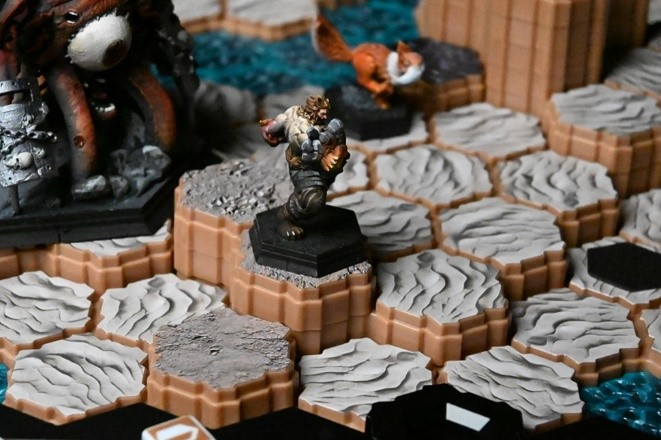
\includegraphics[width=1\linewidth]{chapters//Building/TimeStrikeBuildingRoads.jpg}
    \end{figure}
    \item From there, place the remaining road hexes on any unoccupied basic land hexes adjacent to any other road hexes belonging to the road the unit is standing on.
    \item Roads can be built adjacent to each other regardless of the height difference.
\end{enumerate}

\textit{Note: Roads cannot be built on top of other roads or resource hexes.}

\clearpage
\end{document}